\documentclass[twoside,12pt]{article}
\usepackage{subfiles}
\author{Jakob Teuffel}
%\usepackage{gensymb}
\usepackage{amssymb}
\usepackage{amsmath}

\usepackage{changepage}
%\usepackage{nicefrac}
\usepackage{color}
\usepackage{float}
\usepackage{xparse}
\usepackage{listings}
\usepackage{subfig}
\usepackage{graphicx}
\usepackage{setspace}
\usepackage{afterpage}
\usepackage{centernot}
%\usepackage{scrpage2} 
\usepackage{physics}
%\pagestyle{scrheadings}
\usepackage{breqn}
\usepackage{bbold}
\usepackage{algorithm}
\usepackage[noend]{algpseudocode}
\usepackage{pdfpages}
\usepackage{listings}
\usepackage{xcolor}
\usepackage{ragged2e}
\usepackage{siunitx}
\usepackage[export]{adjustbox}
\usepackage[utf8]{inputenc}
\usepackage{expl3}[2012-07-08]
\ExplSyntaxOn
\cs_if_exist:NF \fpeval { \cs_new_eq:NN \fpeval \fp_eval:n }
\ExplSyntaxOff

%Code Import Options 
\definecolor{codegreen}{rgb}{0,0.6,0}
\definecolor{codegray}{rgb}{0.5,0.5,0.5}
\definecolor{codepurple}{rgb}{0.58,0,0.82}
\lstdefinestyle{mystyle}{
    basicstyle=\ttfamily\fontsize{6}{7}\selectfont,
    commentstyle=\color{codegreen},
    keywordstyle=\color{magenta},
    numberstyle=\tiny\color{codegray},
    stringstyle=\color{codepurple},
    breakatwhitespace=false,         
    %breaklines=true,                 
    captionpos=b,                    
    keepspaces=true,                 
    numbers=left,                    
    numbersep=6pt,                  
    showspaces=false,                
    showstringspaces=false,
    showtabs=false,                  
    tabsize=2
}
\lstset{style=mystyle,
        language=[11]c++,
        inputencoding=utf8,
        extendedchars=true,
    literate=%
        {©}{{\textsuperscript{\textcopyright}}}1
        {²}{{\textsuperscript{2}}}1
}

% UHH Style options
\usepackage[T1]{fontenc}
%\setmainfont{Times New Roman}
\usepackage{setspace}
\onehalfspacing

% Biblography
\usepackage[backend=biber]{biblatex}
\addbibresource{BIB.bib}

%Define Style
\usepackage{geometry}
\geometry{a4paper, portrait ,
 total={210mm , 297mm},
left = 2.5cm,
right = 2.5cm,
bottom = 2.0 cm,
top = 2.0 cm
}
\setlength{\parindent}{0cm}
\usepackage[format=plain,
   font=footnotesize,
   labelfont={bf,it},
   textfont=it]{caption}
\usepackage[justification=centering]{caption}
\makeatletter
\renewcommand\paragraph{\@startsection{paragraph}{4}{\z@}%
  {-3.25ex\@plus -1ex \@minus -.2ex}%
  {1.5ex \@plus .2ex}%
  {\normalfont\normalsize\bfseries}}
\makeatother
\newcommand\mypagebreak{
\vspace*{\fill}
\pagebreak
}

%Index levels 
\setcounter{secnumdepth}{5}
\setcounter{tocdepth}{5}

% Error remark 
\newcommand\Error[1]{\textcolor{red}{\textbf{#1}}}
\usepackage{hyperref}
\hypersetup{
    %PDF
    colorlinks=true,
    %Print
    %colorlinks=false,
    linkcolor=blue,
    filecolor=magenta,      
    urlcolor=cyan,
    pdftitle={Overleaf Example},
    pdfpagemode=FullScreen,
}

% Ref Handling
\newcommand\figref[1]{\textit{\textbf{Figure  \ref{#1}}}}
\newcommand\secref[1]{\textbf{Section \ref{#1}}}
% Vectors as Bold
\renewcommand\vec{\mathbf}

\begin{document}
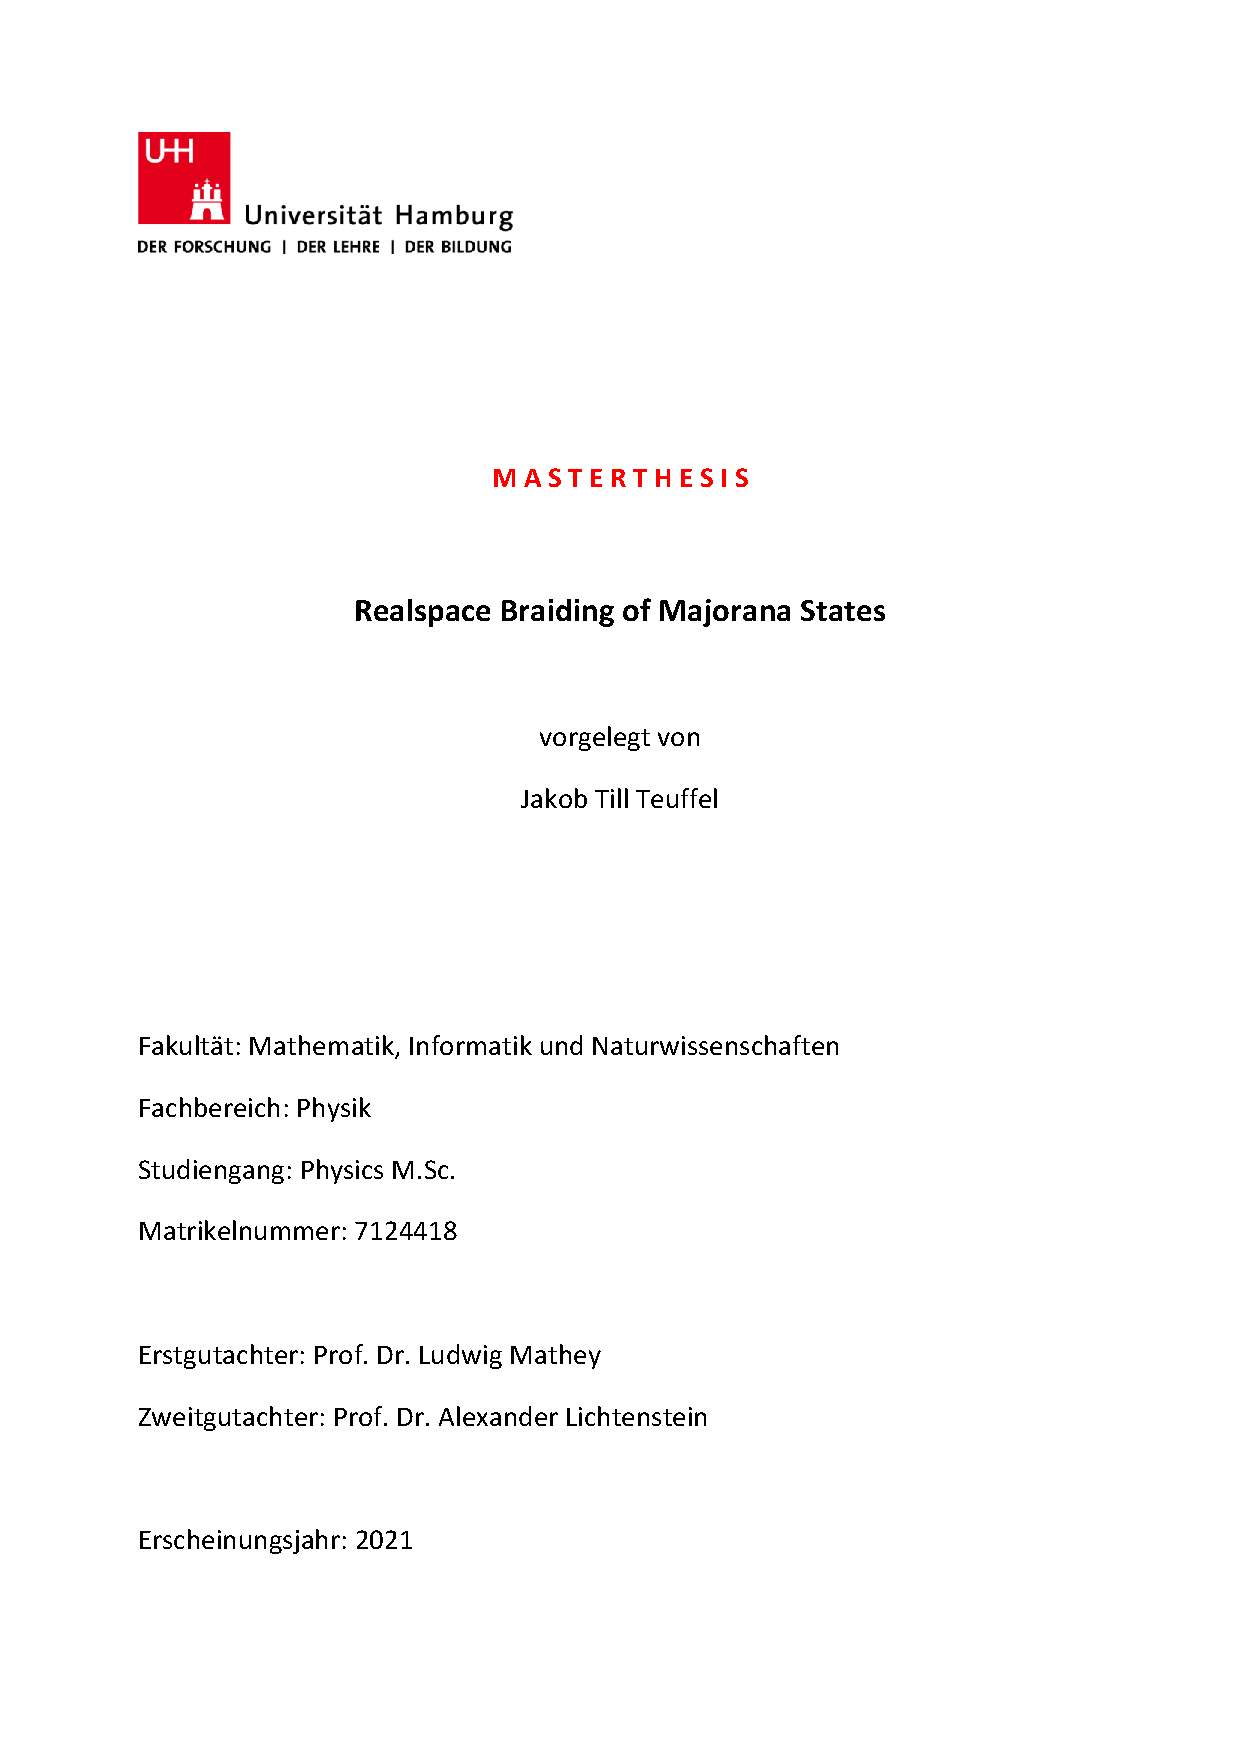
\includepdf[pages=-]{Deckblatt.pdf}
\mypagebreak
\tableofcontents
%\Pend
\listoffigures
\mypagebreak
\mypagebreak
\subfile{Abstract}
\mypagebreak
\subfile{Introduction}
\mypagebreak
\subfile{NonAbelianAnyons}
\mypagebreak
\subfile{topological}
\mypagebreak
\subfile{Numerics}
\mypagebreak
\subfile{Majorana}
\mypagebreak
\subfile{Aufgabenstellung}
\mypagebreak
\subfile{ChiralTopPSuperCond}
\mypagebreak
\section{Analytical Setup}
\subfile{BdG}
\mypagebreak
\subfile{TimeEvolution}
\mypagebreak
\subfile{Numeric_Implementation}
\mypagebreak
\subfile{Results}
\mypagebreak
\subfile{discussion}
\mypagebreak
\section{References}
\printbibliography[heading=subbibliography, title={References}]
\mypagebreak
\subfile{Danksagung}
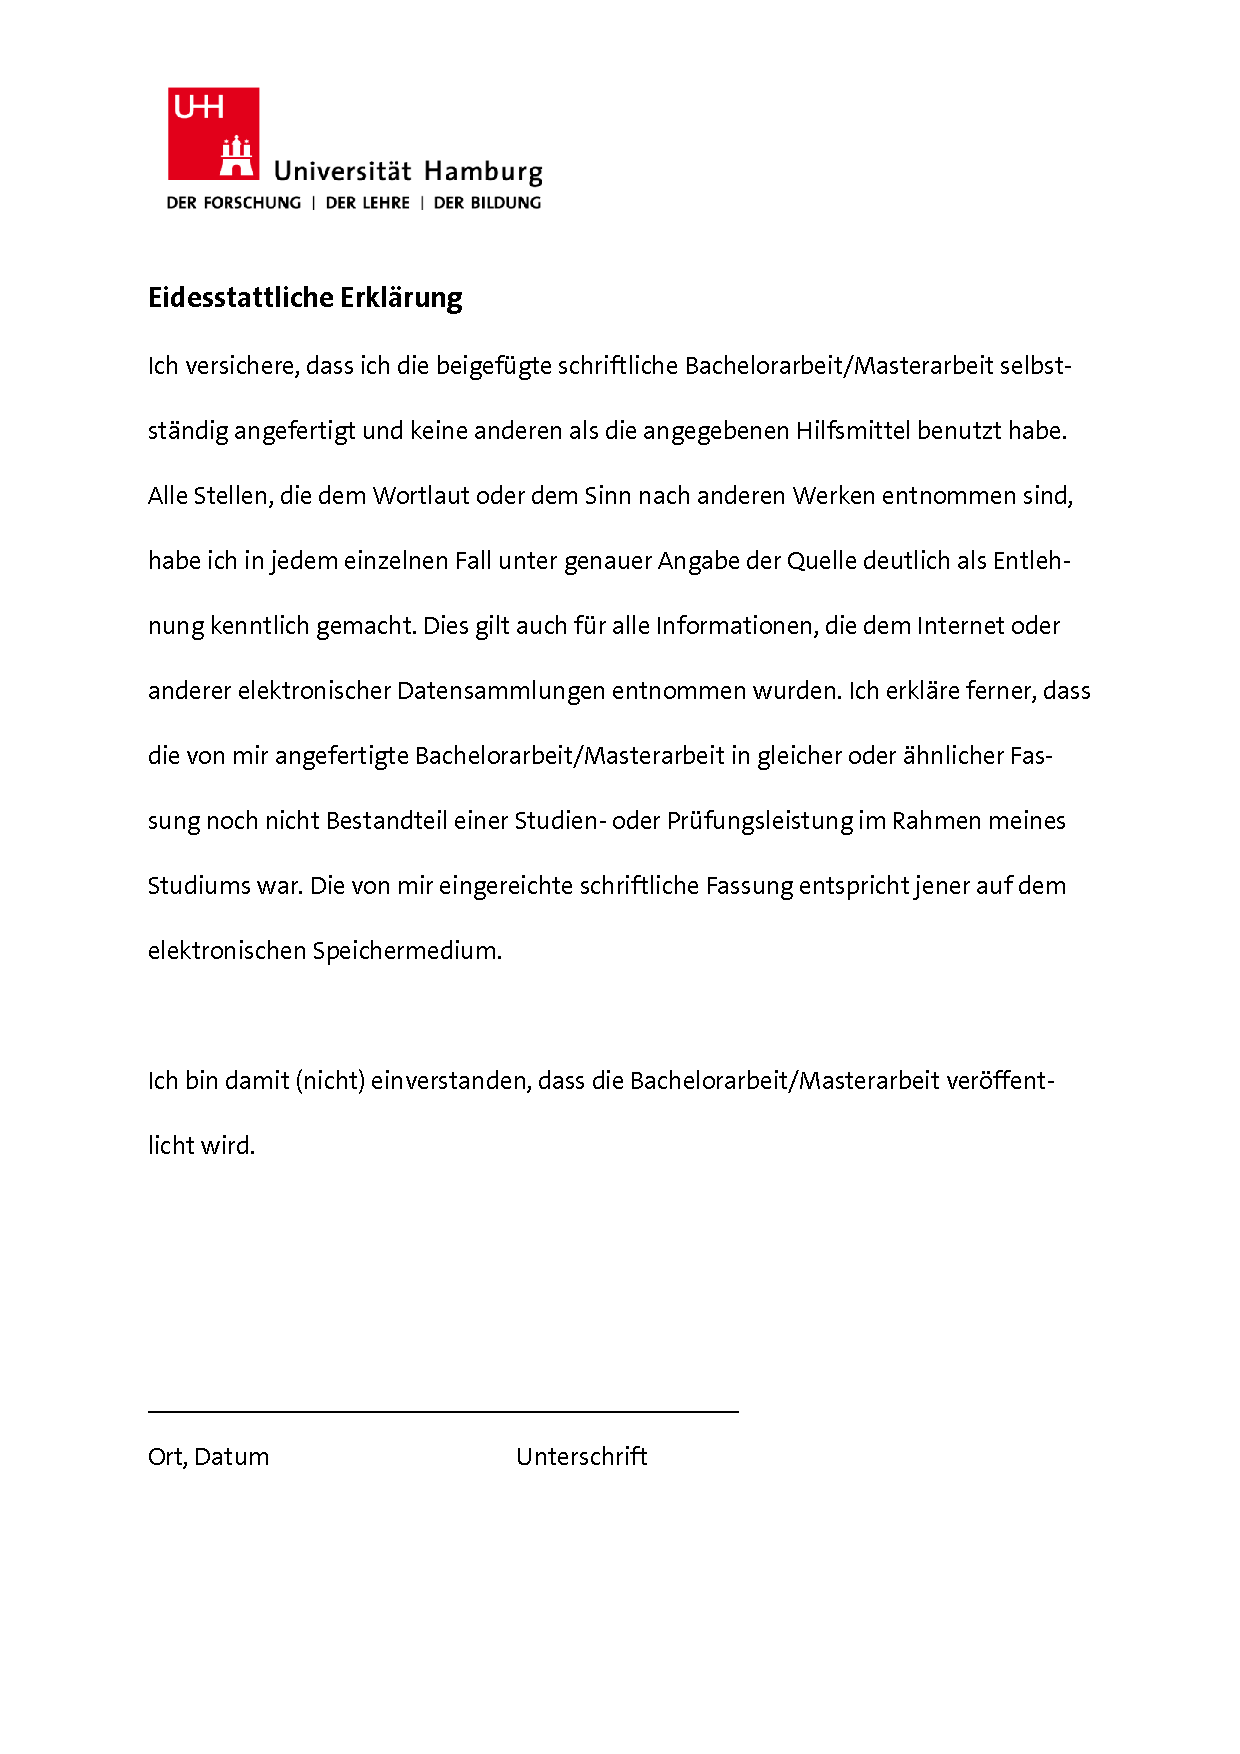
\includepdf[pages=-]{eidesstattlicheerklaerung.pdf}
\subfile{Appendix}
\mypagebreak
\subfile{Appendixc}

\end{document}

%\Error{DEPRECATED}
%\subfile{Time-Evolution}
%\mypagebreak
%\subfile{hamil}